\documentclass[UTF8,a4paper,11pt]{ctexart}

\usepackage{amsmath,amssymb}
\usepackage{booktabs}
\usepackage{caption}
\usepackage{subcaption}
\usepackage{enumitem}
\usepackage{float}
\usepackage{geometry}
\usepackage{graphicx}
\usepackage{hyperref}
\usepackage{longtable}
\usepackage{xcolor}

\geometry{left=2.4cm,right=2.4cm,top=2.5cm,bottom=2.5cm}
\graphicspath{
  {../results/figures/}
  {../Enhanced/results/figures/}
  {../Visual/figures/}
}
\hypersetup{
  colorlinks=true,
  linkcolor=blue!55!black,
  citecolor=blue!55!black,
  urlcolor=blue!55!black
}
\captionsetup{font=small,labelfont=bf}
\setlist[itemize]{leftmargin=2em}
\setlist[enumerate]{leftmargin=2em}
\emergencystretch=2em

\title{\textbf{第二部分：Batch Normalization 实验报告}}
\author{神经网络与深度学习 Project 2}
\date{\today}

\begin{document}
\maketitle

\begin{abstract}
本报告只对应 Project 2 的第二部分 Batch Normalization。实验以 CIFAR-10 图像分类为任务，比较标准 VGG-A 与在每个卷积层后加入 Batch Normalization 的 VGG-A-BN。我们首先完成 BN 层的结构实现与基础训练对比，然后按照作业要求从损失包络、学习率敏感性和梯度变化三个角度分析 BN 对优化过程的影响。基础实验表明，在学习率 $10^{-3}$ 下，VGG-A-BN 的最佳验证准确率达到 $82.18\%$，高于无 BN 模型的 $77.97\%$；在学习率 $2\times10^{-3}$ 下，无 BN 模型退化到接近随机猜测的 $10.00\%$，而 BN 模型仍达到 $81.36\%$。跨学习率的 loss landscape 包络宽度从无 BN 的平均 $1.900$ 降至 BN 的 $0.375$，约减少 $80.3\%$。这些结果说明，BN 的主要贡献不只是提升最终精度，更重要的是改善优化稳定性、扩大可用学习率范围，并使训练过程对超参数变化更鲁棒。
\end{abstract}

\tableofcontents
\newpage

\section{实验目标与代码结构}

本部分任务要求比较带 BN 与不带 BN 的 VGG-A，并进一步分析 BN 如何帮助优化。围绕这一目标，本实验完成了三类工作。

第一，基于提供的 \texttt{codes/VGG\_BatchNorm} 脚手架，在 \texttt{Batch\_Normalization} 中实现了可独立运行的实验代码。核心文件包括：
\begin{itemize}
  \item \texttt{models.py}：实现 CIFAR-10 输入尺寸下的 VGG-A 与 VGG-A-BatchNorm；
  \item \texttt{data\_utils.py}：实现 CIFAR-10 数据加载、归一化与子集调试；
  \item \texttt{run\_bn\_experiments.py}：实现训练、验证、loss 记录、梯度范数记录和 loss landscape 包络图生成。
\end{itemize}

第二，在 \texttt{Batch\_Normalization/Enhanced} 中补充学习率敏感性与梯度预测性实验，用于从优化角度进一步解释 BN 的作用。

第三，在 \texttt{Batch\_Normalization/Visual} 中构建报告级可视化脚本，基于基础实验结果与已保存 checkpoint 生成训练曲线、三维 loss surface 以及激活分布 ridgeline 图。所有可视化均围绕基础 BN 实验，不使用额外模型结构的扩展结果。

\section{Batch Normalization 方法}

\subsection{BN 的计算形式}

本实验关注卷积神经网络中的二维 Batch Normalization。设某一 BN 层输入为四维张量 $I_{b,c,x,y}$，其中 $b$ 表示 mini-batch 内样本编号，$c$ 表示通道，$x,y$ 表示空间位置。BN 对同一通道的所有 batch 与空间位置共同统计均值和方差：
\begin{equation}
  \mu_c = \frac{1}{|\mathcal{B}|}\sum_{b,x,y} I_{b,c,x,y},
\end{equation}
\begin{equation}
  \sigma_c^2 = \frac{1}{|\mathcal{B}|}\sum_{b,x,y}(I_{b,c,x,y}-\mu_c)^2.
\end{equation}
随后进行标准化和可学习仿射变换：
\begin{equation}
  O_{b,c,x,y}
  =
  \gamma_c
  \frac{I_{b,c,x,y}-\mu_c}{\sqrt{\sigma_c^2+\epsilon}}
  + \beta_c .
\end{equation}
其中 $\gamma_c,\beta_c$ 是可学习参数。训练阶段使用当前 mini-batch 的统计量，同时维护 running mean 和 running variance；测试阶段使用训练过程中累计得到的 running statistics。

\subsection{VGG-A 与 VGG-A-BN 实现}

基础网络采用适配 CIFAR-10 的 VGG-A。输入图像大小为 $32\times32\times3$，卷积部分的通道配置为
\[
64,\ M,\ 128,\ M,\ 256,\ 256,\ M,\ 512,\ 512,\ M,\ 512,\ 512,\ M,
\]
其中 $M$ 表示 $2\times2$ max pooling。卷积部分最终输出 $512\times1\times1$ 特征，再经过三层全连接分类器：
\[
512 \rightarrow 512 \rightarrow 512 \rightarrow 10.
\]

无 BN 模型采用标准结构
\[
\mathrm{Conv2d} \rightarrow \mathrm{ReLU}.
\]
带 BN 模型在每个卷积层后加入 BN：
\[
\mathrm{Conv2d} \rightarrow \mathrm{BatchNorm2d} \rightarrow \mathrm{ReLU}.
\]
由于 BN 层已经包含可学习的平移与缩放参数，带 BN 的卷积层不使用 bias。参数量方面，VGG-A 有 $9{,}750{,}922$ 个参数，VGG-A-BN 有 $9{,}753{,}674$ 个参数。二者参数量几乎一致，因此性能差异主要来自 BN 对训练动态和优化过程的影响，而不是模型容量显著增加。

\section{基础实验设置}

\subsection{数据集与预处理}

所有实验均在 CIFAR-10 上进行。训练集包含 $50{,}000$ 张图像，测试集包含 $10{,}000$ 张图像。输入图像先转换为 tensor，再按 CIFAR-10 经验均值和标准差归一化：
\[
\mu=(0.4914,0.4822,0.4465),\qquad
\sigma=(0.2470,0.2435,0.2616).
\]
基础 BN 实验默认不使用随机裁剪、随机翻转等数据增强，因为本部分重点是比较 BN 对优化过程的影响，而不是追求最高分类精度。

\subsection{训练配置}

基础训练配置见表~\ref{tab:base_config}。为保证对比公平，BN 与 no-BN 使用完全相同的优化器、batch size、epoch 数、随机种子和学习率列表。

\begin{table}[H]
  \centering
  \caption{基础 BN 对比实验配置}
  \label{tab:base_config}
  \begin{tabular}{ll}
    \toprule
    项目 & 设置 \\
    \midrule
    数据集 & CIFAR-10 \\
    模型 & VGG-A / VGG-A-BatchNorm \\
    Epoch & 20 \\
    Batch size & 128 \\
    优化器 & Adam \\
    Weight decay & $5\times10^{-4}$ \\
    学习率 & $10^{-3},\,2\times10^{-3},\,5\times10^{-4},\,10^{-4}$ \\
    随机种子 & 2020 \\
    数据增强 & 无 \\
    \bottomrule
  \end{tabular}
\end{table}

每次训练均记录每个 batch 的训练 loss、每个 epoch 的训练准确率与验证准确率，并保存 \texttt{best.pt} 与 \texttt{last.pt}。这些结果用于后续 loss landscape、可视化和报告分析。

\section{VGG-A 与 VGG-A-BN 基础对比}

\subsection{主要分类结果}

表~\ref{tab:base_results} 总结了四组学习率下 no-BN 与 BN 的训练结果。可以看到，BN 在中等和偏大学习率下优势明显，尤其是 $2\times10^{-3}$ 时，无 BN 模型训练失败，验证准确率停留在随机分类水平；而 BN 模型仍然取得 $81.36\%$ 的最佳验证准确率。

\begin{table}[H]
  \centering
  \caption{基础实验中不同学习率下 VGG-A 与 VGG-A-BN 的性能对比}
  \label{tab:base_results}
  \begin{tabular}{ccccc}
    \toprule
    学习率 & 模型 & 最佳验证准确率 & 最佳 epoch & 最终验证准确率 \\
    \midrule
    $10^{-4}$ & VGG-A & $76.84\%$ & 13 & $76.28\%$ \\
    $10^{-4}$ & VGG-A-BN & $74.71\%$ & 17 & $74.34\%$ \\
    $5\times10^{-4}$ & VGG-A & $79.25\%$ & 19 & $78.12\%$ \\
    $5\times10^{-4}$ & VGG-A-BN & $81.82\%$ & 19 & $78.17\%$ \\
    $10^{-3}$ & VGG-A & $77.97\%$ & 18 & $77.79\%$ \\
    $10^{-3}$ & VGG-A-BN & $\mathbf{82.18\%}$ & 12 & $\mathbf{81.03\%}$ \\
    $2\times10^{-3}$ & VGG-A & $10.00\%$ & 1 & $10.00\%$ \\
    $2\times10^{-3}$ & VGG-A-BN & $81.36\%$ & 19 & $79.53\%$ \\
    \bottomrule
  \end{tabular}
\end{table}

从平均表现看，四个学习率下 no-BN 的平均最佳验证准确率为 $61.02\%$，BN 为 $80.02\%$。由于 no-BN 在 $2\times10^{-3}$ 下完全失效，这一平均值差距很大。若只观察正常收敛的学习率，BN 在 $5\times10^{-4}$ 和 $10^{-3}$ 下也分别带来 $2.57$ 和 $4.21$ 个百分点的最佳准确率提升。

\subsection{训练曲线分析}

图~\ref{fig:training_curves} 展示了学习率 $10^{-3}$ 下的训练 loss 和验证准确率变化。BN 模型从第一个 epoch 开始就表现出更快的优化速度：第 1 个 epoch 后，BN 的验证准确率达到 $60.89\%$，而 no-BN 为 $36.96\%$；第 3 个 epoch 后，BN 已达到 $74.66\%$，no-BN 为 $60.28\%$。最终 BN 在第 12 个 epoch 达到最高验证准确率 $82.18\%$，比 no-BN 的最高点更早出现。

\begin{figure}[H]
  \centering
  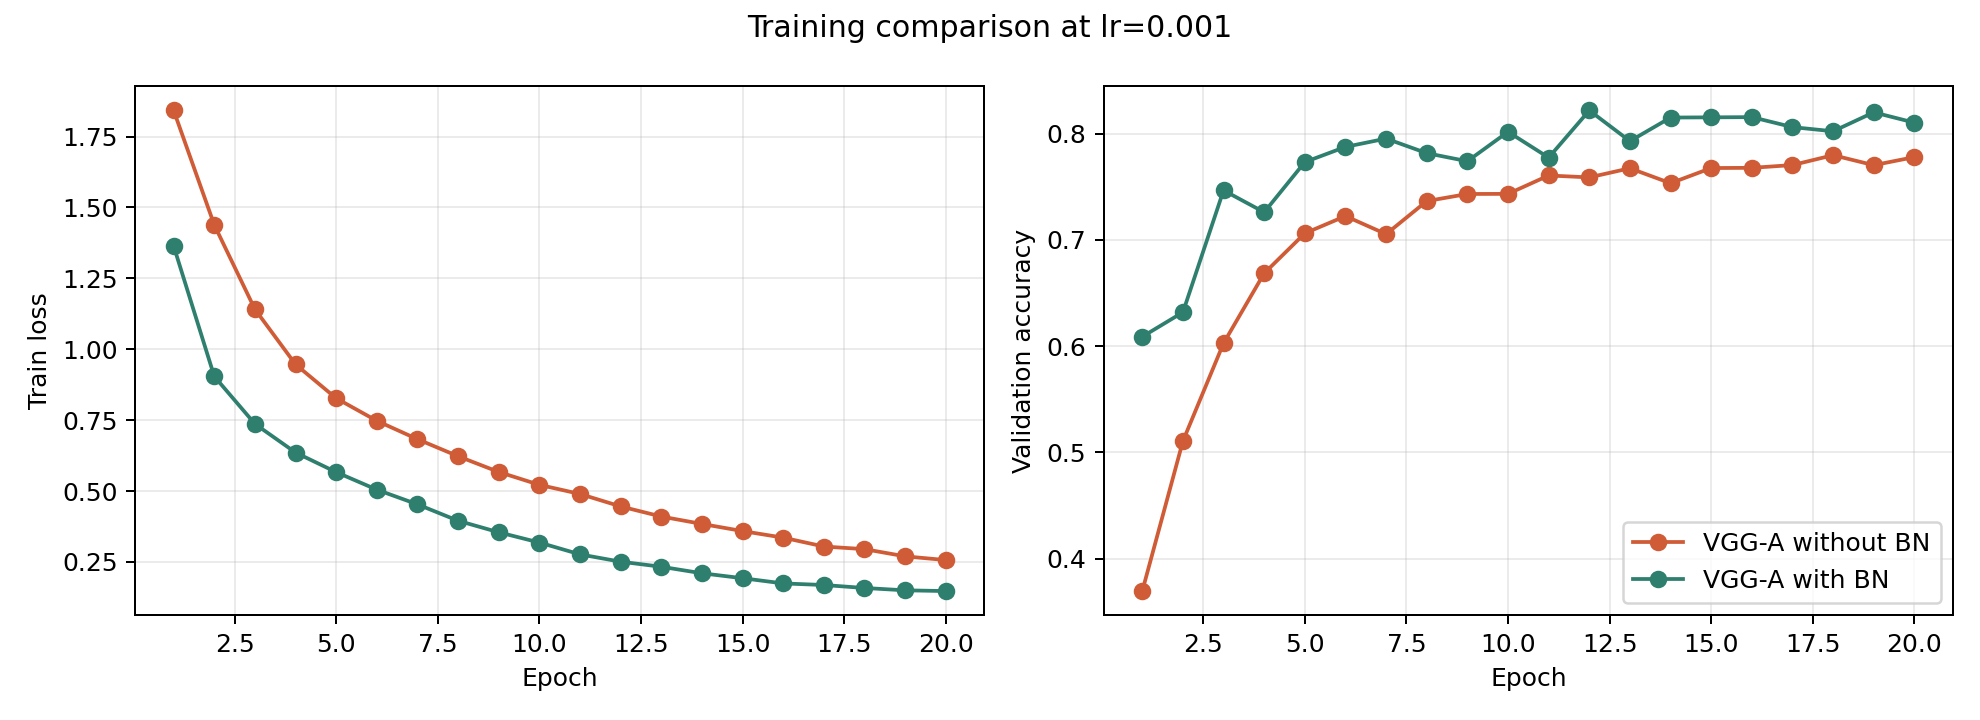
\includegraphics[width=0.95\linewidth]{training_curves_first_lr.png}
  \caption{学习率 $10^{-3}$ 下 VGG-A 与 VGG-A-BN 的训练 loss 与验证准确率对比。BN 模型收敛更快，并在较早 epoch 达到更高验证准确率。}
  \label{fig:training_curves}
\end{figure}

这一结果说明 BN 在本实验中不仅提高了最终精度，而且改变了训练早期的优化动态，使网络更快进入有效分类状态。

\section{BN 对 Loss Landscape 的影响}

\subsection{包络式 loss landscape 度量}

作业说明建议选择多组学习率，并在同一训练 step 上统计不同学习率下 loss 的最大值与最小值，形成
\[
\mathrm{max\_curve}(t)=\max_i L_i(t),\qquad
\mathrm{min\_curve}(t)=\min_i L_i(t),
\]
其中 $i$ 表示不同学习率的训练 run。两条曲线之间的区域可理解为在不同步长下训练 loss 的波动包络。包络越宽，说明训练过程对学习率变化越敏感；包络越窄，说明优化过程更稳定。

图~\ref{fig:loss_landscape_envelope} 展示了 no-BN 与 BN 的 loss 包络对比。无 BN 模型的包络长期覆盖到交叉熵约 $2.3$ 附近，这是因为 $2\times10^{-3}$ 学习率下模型几乎停留在随机猜测状态。相比之下，BN 模型的 loss 区域更低且更窄，说明不同学习率下的训练行为更加一致。

\begin{figure}[H]
  \centering
  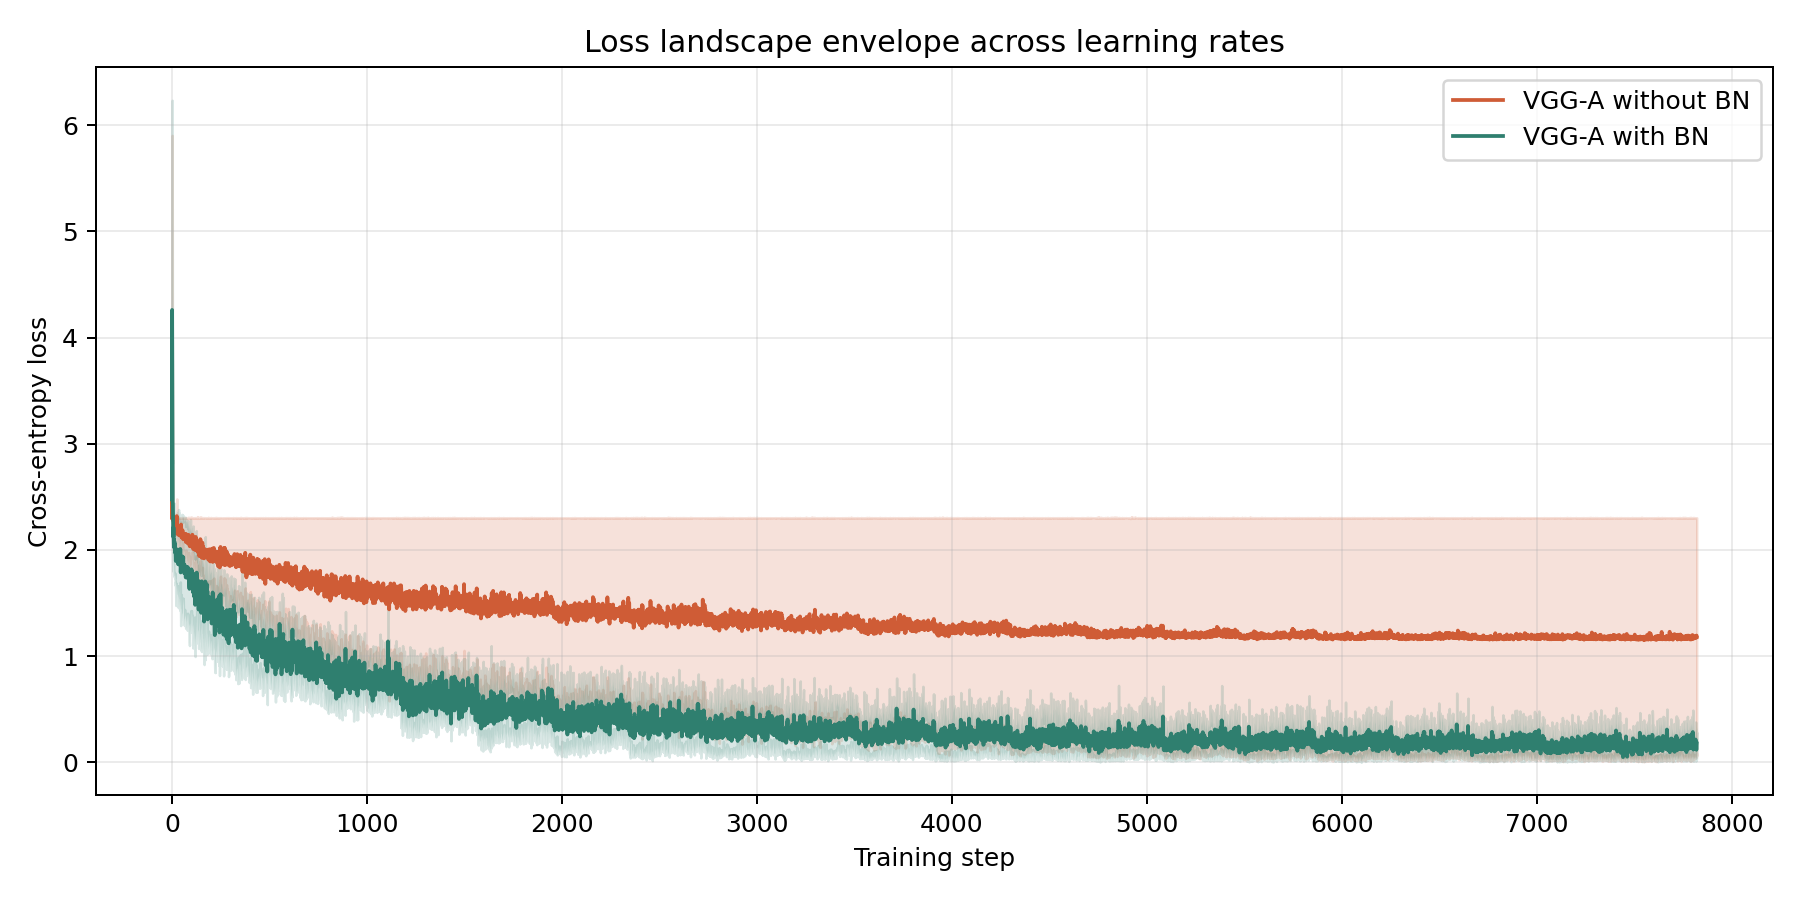
\includegraphics[width=0.95\linewidth]{loss_landscape_envelope.png}
  \caption{跨学习率 loss landscape 包络。BN 显著缩小不同学习率训练曲线之间的 loss 波动范围。}
  \label{fig:loss_landscape_envelope}
\end{figure}

\subsection{包络宽度定量分析}

表~\ref{tab:landscape_width} 给出了包络宽度的统计量。BN 的平均包络宽度为 $0.375$，无 BN 为 $1.900$；BN 的平均宽度约为 no-BN 的 $19.7\%$，即缩小约 $80.3\%$。中位数宽度也从 $2.077$ 降至 $0.355$。

\begin{table}[H]
  \centering
  \caption{Loss landscape 包络宽度统计}
  \label{tab:landscape_width}
  \begin{tabular}{ccccc}
    \toprule
    模型 & 平均宽度 & 中位数宽度 & 90 分位宽度 & 最大宽度 \\
    \midrule
    VGG-A & $1.900$ & $2.077$ & $2.262$ & $3.603$ \\
    VGG-A-BN & $\mathbf{0.375}$ & $\mathbf{0.355}$ & $\mathbf{0.564}$ & $3.948$ \\
    \bottomrule
  \end{tabular}
\end{table}

最大宽度上 BN 略高，主要来自训练初期个别 batch 的尖峰；但从平均、中位数和 90 分位数看，BN 的整体包络显著更窄。更重要的是，BN 包络的平均上界为 $0.591$，而 no-BN 的平均上界为 $2.303$，这直接反映了 no-BN 在某些学习率下无法有效优化。

\section{学习率敏感性扩展实验}

\subsection{实验设计}

为了系统验证 BN 是否扩大可用学习率范围，我们进一步在 \texttt{Enhanced} 中运行学习率 sweep。学习率列表扩展为
\[
5\times10^{-5},\ 10^{-4},\ 5\times10^{-4},\ 10^{-3},\ 2\times10^{-3},\ 3\times10^{-3},\ 5\times10^{-3}.
\]
其他设置保持不变：CIFAR-10、20 epoch、batch size 128、Adam、weight decay $5\times10^{-4}$、无数据增强。

\subsection{结果}

表~\ref{tab:lr_sweep} 与图~\ref{fig:lr_sensitivity} 显示了不同学习率下的最佳验证准确率。BN 的表现随学习率变化更平滑：其最佳准确率在 $70.58\%$ 至 $82.18\%$ 之间，标准差为 $0.041$；no-BN 的范围为 $10.00\%$ 至 $79.25\%$，标准差为 $0.296$。

\begin{table}[H]
  \centering
  \caption{学习率敏感性实验结果}
  \label{tab:lr_sweep}
  \begin{tabular}{cccc}
    \toprule
    学习率 & VGG-A 最佳准确率 & VGG-A-BN 最佳准确率 & BN 提升 \\
    \midrule
    $5\times10^{-5}$ & $75.09\%$ & $70.58\%$ & $-4.51$ pp \\
    $10^{-4}$ & $76.84\%$ & $74.71\%$ & $-2.13$ pp \\
    $5\times10^{-4}$ & $79.25\%$ & $81.82\%$ & $+2.57$ pp \\
    $10^{-3}$ & $77.97\%$ & $\mathbf{82.18\%}$ & $+4.21$ pp \\
    $2\times10^{-3}$ & $10.00\%$ & $81.36\%$ & $+71.36$ pp \\
    $3\times10^{-3}$ & $10.00\%$ & $79.46\%$ & $+69.46$ pp \\
    $5\times10^{-3}$ & $65.49\%$ & $75.00\%$ & $+9.51$ pp \\
    \bottomrule
  \end{tabular}
\end{table}

\begin{figure}[H]
  \centering
  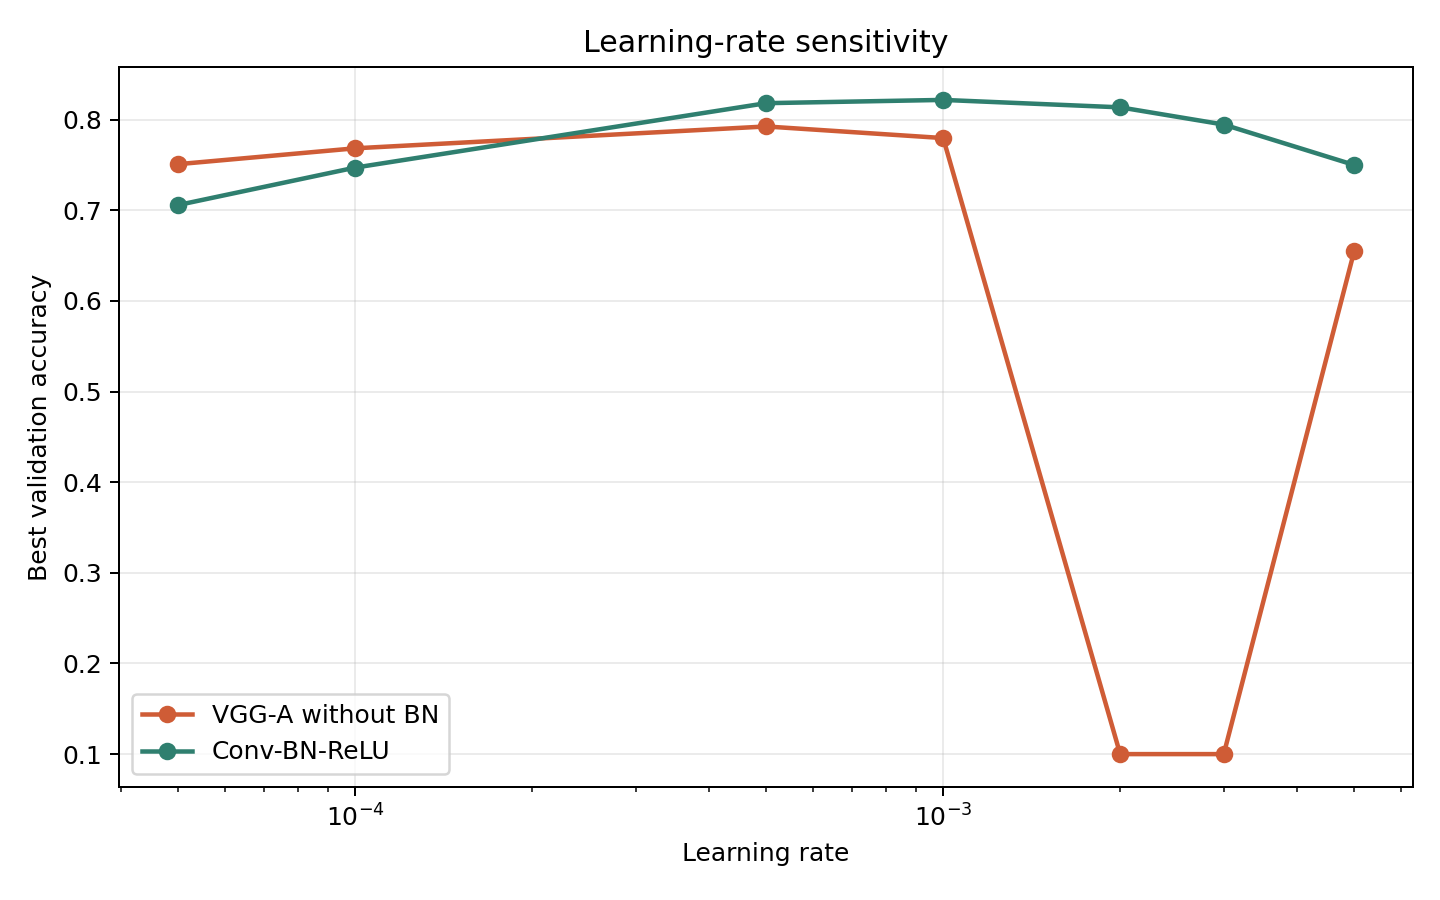
\includegraphics[width=0.78\linewidth]{lr_sensitivity.png}
  \caption{学习率敏感性曲线。BN 在 $5\times10^{-4}$ 至 $5\times10^{-3}$ 区间保持较高准确率，而无 BN 在 $2\times10^{-3}$ 和 $3\times10^{-3}$ 下明显失效。}
  \label{fig:lr_sensitivity}
\end{figure}

这一结果支持如下判断：BN 的优势在小学习率下并不必然体现，因为此时优化步长较保守，标准 VGG-A 也能稳定下降；但当学习率增大时，BN 显著提高了训练鲁棒性，使模型能够承受更大的参数更新。

\section{梯度预测性分析}

\subsection{度量定义}

为了进一步接近作业中提到的 ``gradient predictiveness''，我们记录相邻 step 的梯度变化。设第 $t$ 步的参数为 $w_t$，梯度为 $g_t=\nabla L(w_t)$，定义：
\begin{equation}
  \Delta_g(t) = \|g_t-g_{t-1}\|_2,
\end{equation}
\begin{equation}
  r_g(t)=\frac{\|g_t-g_{t-1}\|_2}{\|g_{t-1}\|_2+\epsilon},
\end{equation}
\begin{equation}
  c_g(t)=
  \frac{g_t^\top g_{t-1}}{\|g_t\|_2\|g_{t-1}\|_2+\epsilon},
\end{equation}
以及距离归一化的最大梯度差异：
\begin{equation}
  D_g(t)=\frac{\|g_t-g_{t-1}\|_2}{\|w_t-w_{t-1}\|_2+\epsilon}.
\end{equation}
其中 $r_g$ 越小、$c_g$ 越大，通常表示相邻 step 的梯度方向更一致，局部线性近似更有预测性。

\subsection{结果与解释}

表~\ref{tab:gradient_predictiveness} 展示了 $10^{-3}$ 和 $2\times10^{-3}$ 两个学习率下的梯度统计。需要注意的是，梯度指标本身容易受是否成功训练影响。例如在 $2\times10^{-3}$ 下，无 BN 模型已经退化到随机猜测附近，其梯度范数和梯度变化都很小，这并不代表优化景观良好，而是模型没有进入有效学习状态。因此该表需要结合验证准确率一起解释。

\begin{table}[H]
  \centering
  \caption{梯度预测性统计}
  \label{tab:gradient_predictiveness}
  \begin{tabular}{cccccc}
    \toprule
    学习率 & 模型 & 最佳准确率 & 平均相对梯度变化 & 平均梯度余弦 & 最大 $D_g$ \\
    \midrule
    $10^{-3}$ & VGG-A & $77.97\%$ & $1.338$ & $0.170$ & $79.59$ \\
    $10^{-3}$ & VGG-A-BN & $82.18\%$ & $1.368$ & $0.144$ & $\mathbf{49.46}$ \\
    $2\times10^{-3}$ & VGG-A & $10.00\%$ & $1.490$ & $0.003$ & $21.62$ \\
    $2\times10^{-3}$ & VGG-A-BN & $81.36\%$ & $1.353$ & $0.154$ & $29.59$ \\
    \bottomrule
  \end{tabular}
\end{table}

图~\ref{fig:gradient_predictiveness} 给出了学习率 $10^{-3}$ 下的 rolling mean 曲线。BN 与 no-BN 的相对梯度变化量级接近，但 BN 在有效训练的同时保持了较低的最大 $D_g$。在 $2\times10^{-3}$ 下，更关键的现象是 no-BN 的梯度方向几乎失去连续性，平均余弦仅 $0.003$，且模型准确率停在 $10\%$；BN 则保持 $0.154$ 的平均梯度余弦并正常训练到 $81.36\%$。

\begin{figure}[H]
  \centering
  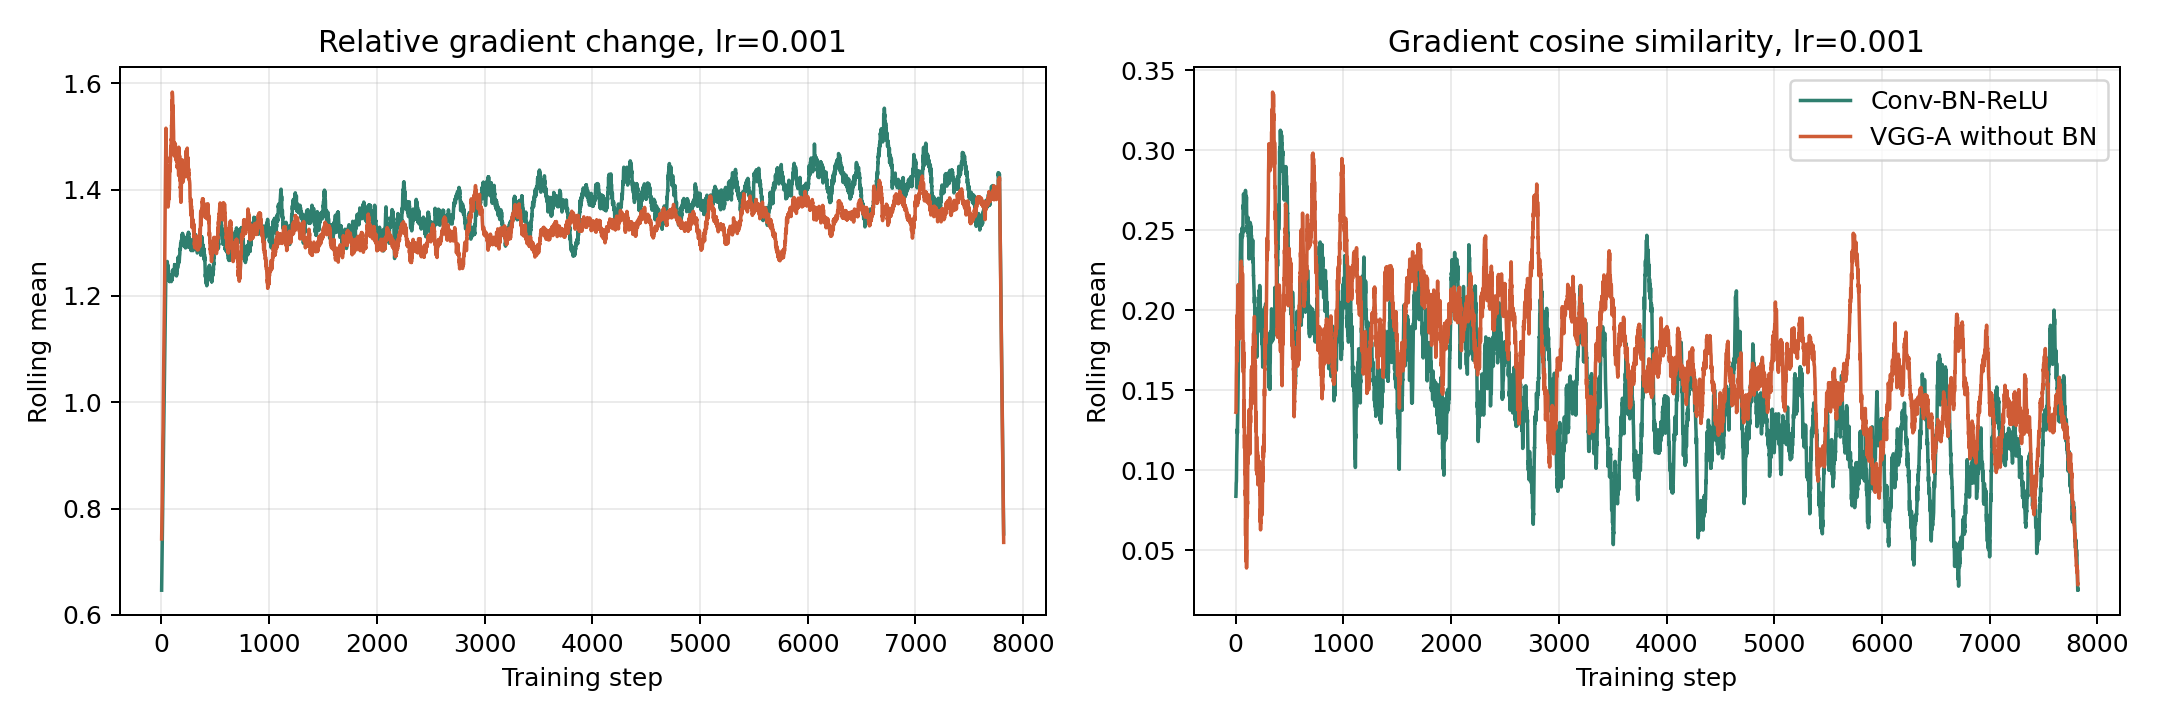
\includegraphics[width=0.95\linewidth]{gradient_predictiveness.png}
  \caption{学习率 $10^{-3}$ 下的相对梯度变化与梯度余弦相似度 rolling mean。梯度指标需要与最终准确率结合解释，避免把训练失败后的低梯度误读为稳定优化。}
  \label{fig:gradient_predictiveness}
\end{figure}

综合来看，梯度预测性实验并不是简单地显示 BN 在所有指标上绝对更小或更大，而是表明 BN 可以在更激进的学习率下维持有效学习，使梯度变化不至于导致训练完全崩溃。这与 loss 包络和学习率 sweep 的结论一致。

\section{增强可视化实验}

\subsection{论文风格训练曲线}

为了更直观地展示 BN 在不同学习率下的稳定性，我们将 $10^{-3}$ 与 $2\times10^{-3}$ 两组学习率的训练/测试准确率放在同一张图中，如图~\ref{fig:paper_accuracy}。其中虚线表示 $2\times10^{-3}$。可以看到，无 BN 在该学习率下训练准确率和测试准确率均长期保持在约 $10\%$；BN 虽然使用相同学习率，却仍能正常上升到约 $80\%$。

\begin{figure}[H]
  \centering
  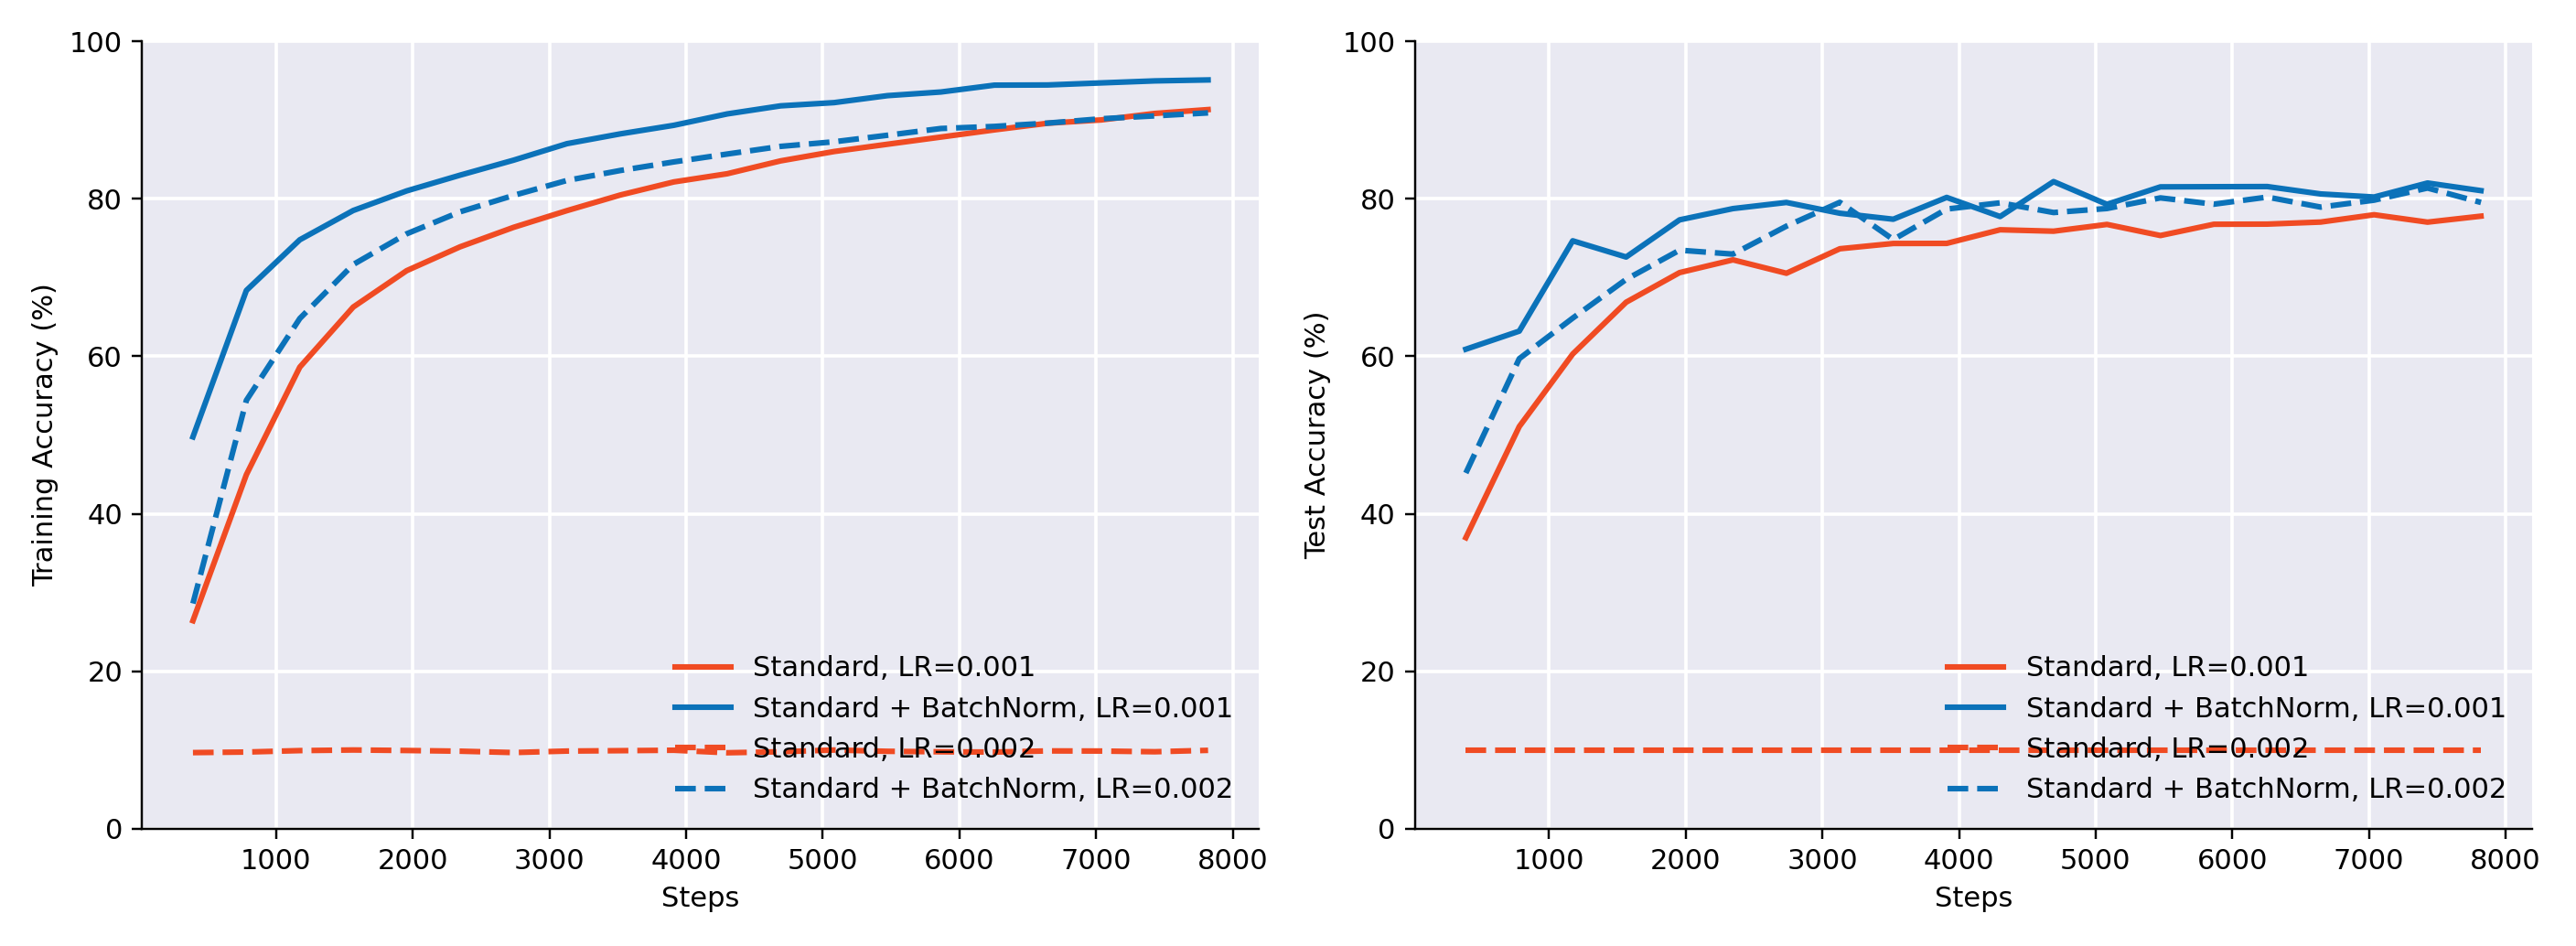
\includegraphics[width=0.95\linewidth]{paper_style_accuracy_panels.png}
  \caption{论文风格训练/测试准确率曲线。该图直接展示了 BN 对较大学习率训练的稳定作用。}
  \label{fig:paper_accuracy}
\end{figure}

\subsection{三维 loss surface 可视化}

除作业要求的 loss 包络外，我们还基于已训练 checkpoint 进行了二维参数切片的三维 loss surface 可视化。具体做法是取学习率 $10^{-3}$ 下的 \texttt{best.pt}，在参数空间中采样两个 filter-normalized random directions $d_1,d_2$，计算：
\[
  L(w+\alpha d_1+\beta d_2),
\]
并在二维网格上绘制 loss surface。该图是高维参数空间的局部二维切片，不代表完整 loss landscape，但可以作为直观补充。

\begin{figure}[H]
  \centering
  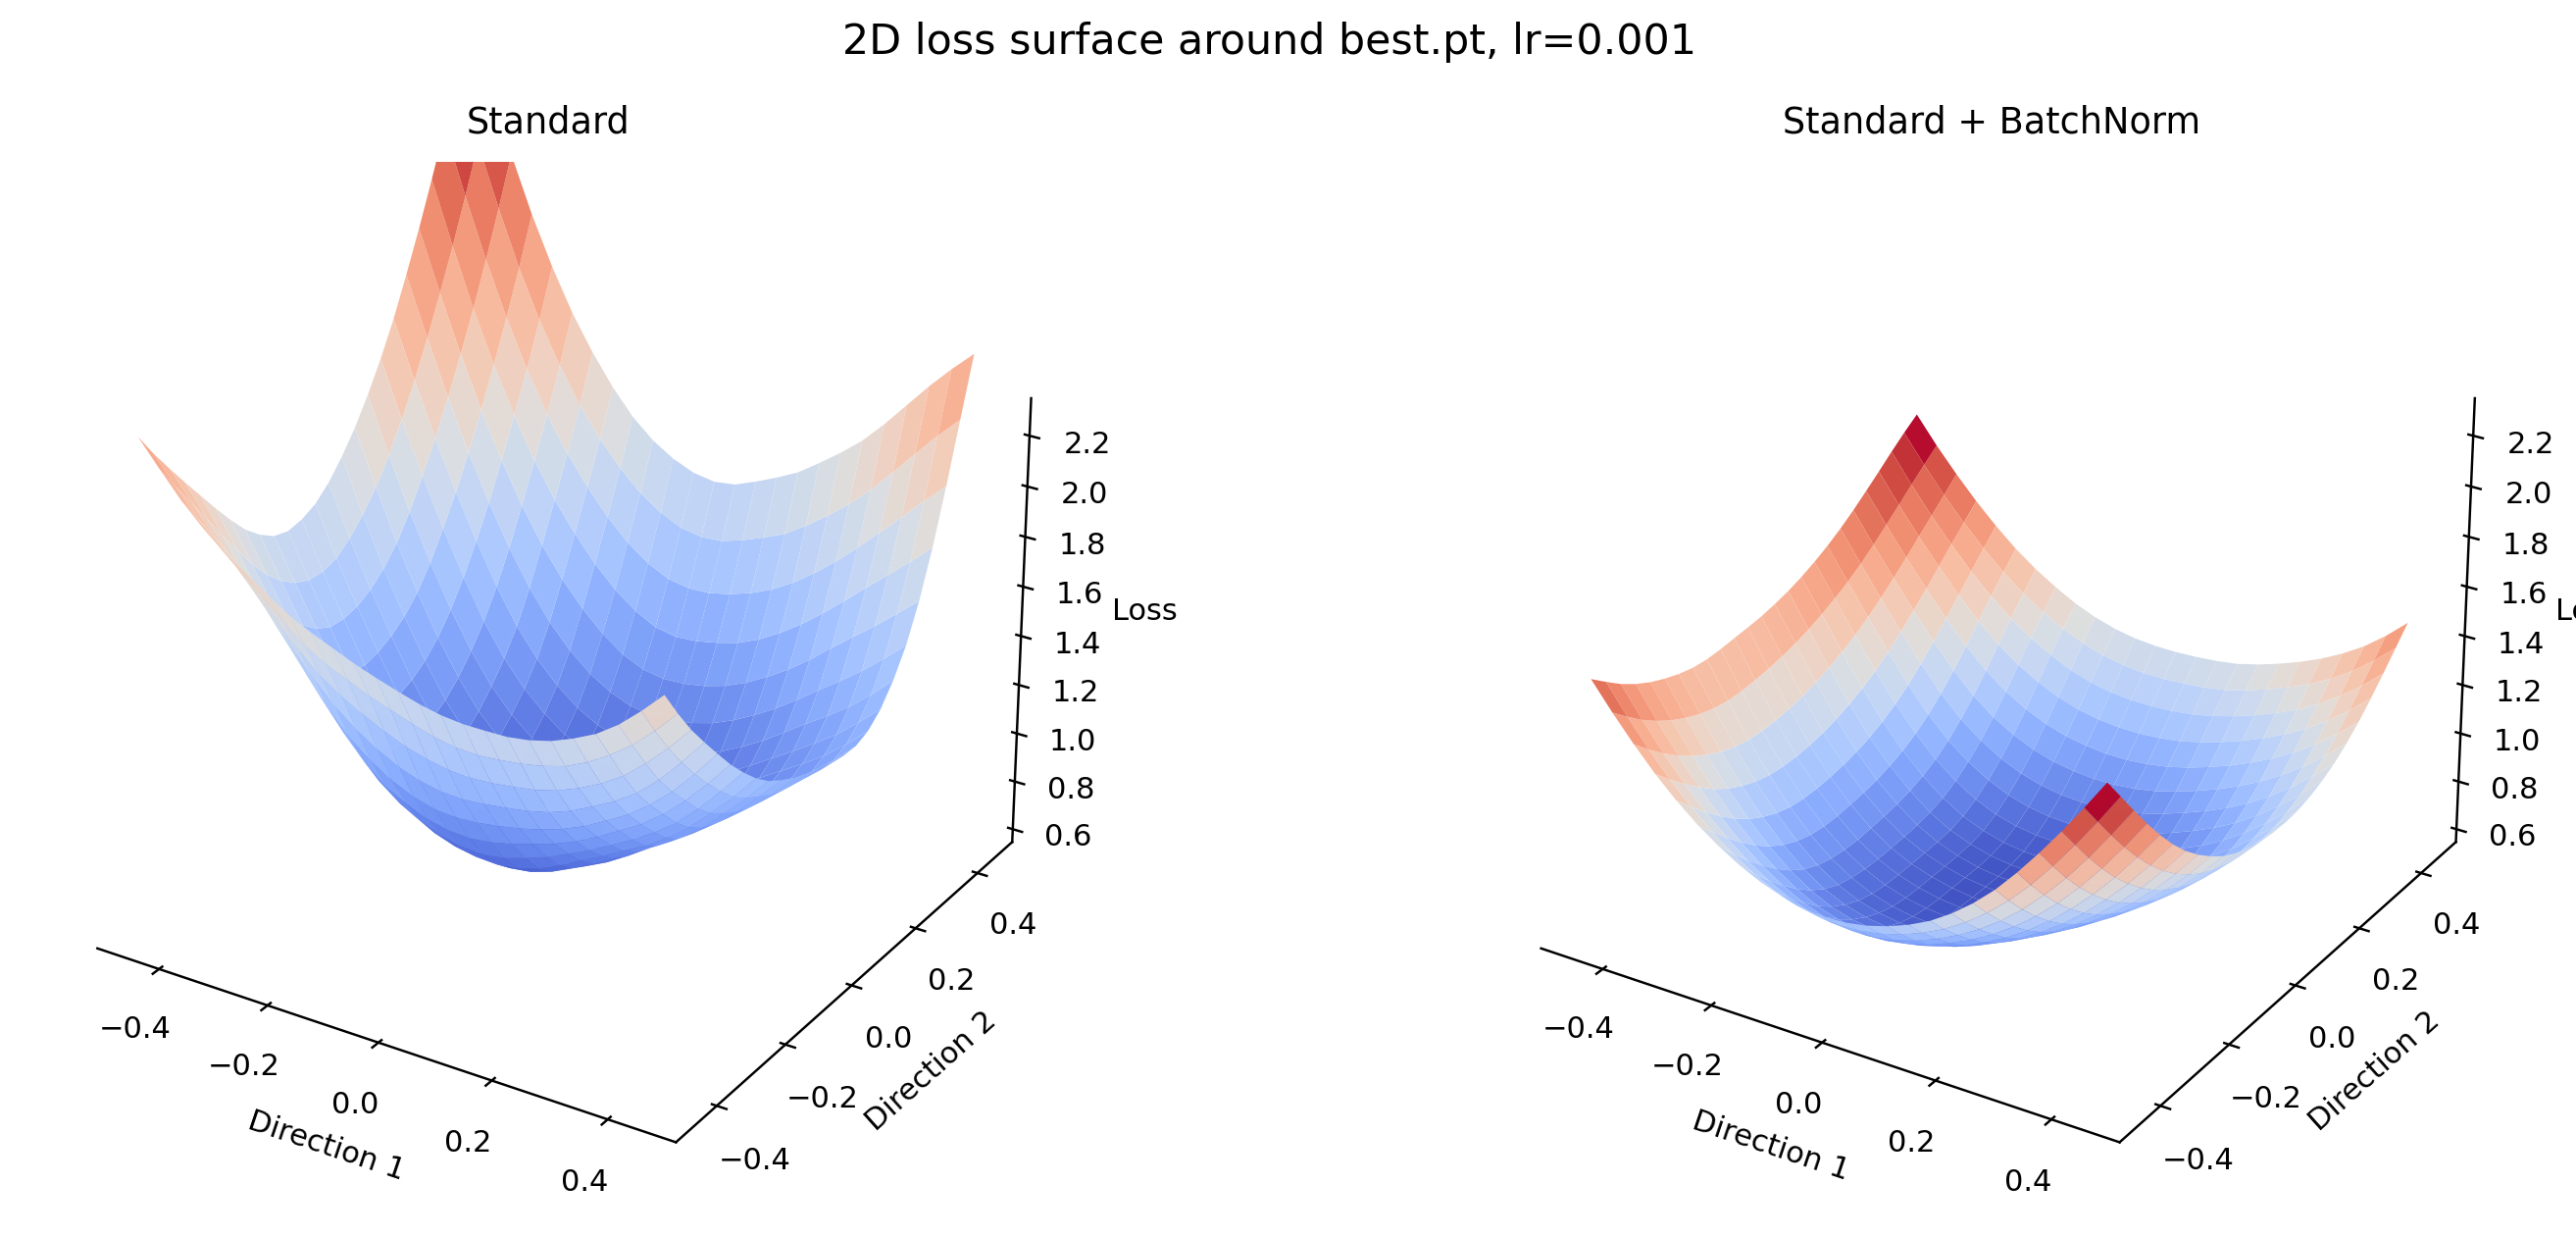
\includegraphics[width=0.95\linewidth]{loss_surface_3d_no_bn_vs_bn.png}
  \caption{学习率 $10^{-3}$、best checkpoint 附近的二维 loss surface。左右图使用相同的采样半径与 z 轴范围，用于直观比较局部曲面形态。}
  \label{fig:loss_surface_3d}
\end{figure}

从图~\ref{fig:loss_surface_3d} 看，两种模型在最优点附近都呈现碗状结构；BN 的曲面并非在任意方向上都更平坦，但低 loss 区域更规整。这也提醒我们：单个二维切片只能作为直观展示，严谨结论仍应以跨学习率 loss 包络和准确率统计为主。

\subsection{激活分布可视化}

BN 的直接作用对象是中间激活分布。因此我们在学习率 $10^{-3}$ 的 best checkpoint 上，对验证集样本进行前向传播，并采集第 1、4、8 个卷积位置附近的激活分布。对 no-BN 模型采集卷积输出；对 BN 模型采集对应 BatchNorm 层输出。图~\ref{fig:activation_distribution} 展示了不同通道的 ridgeline 分布。

\begin{figure}[H]
  \centering
  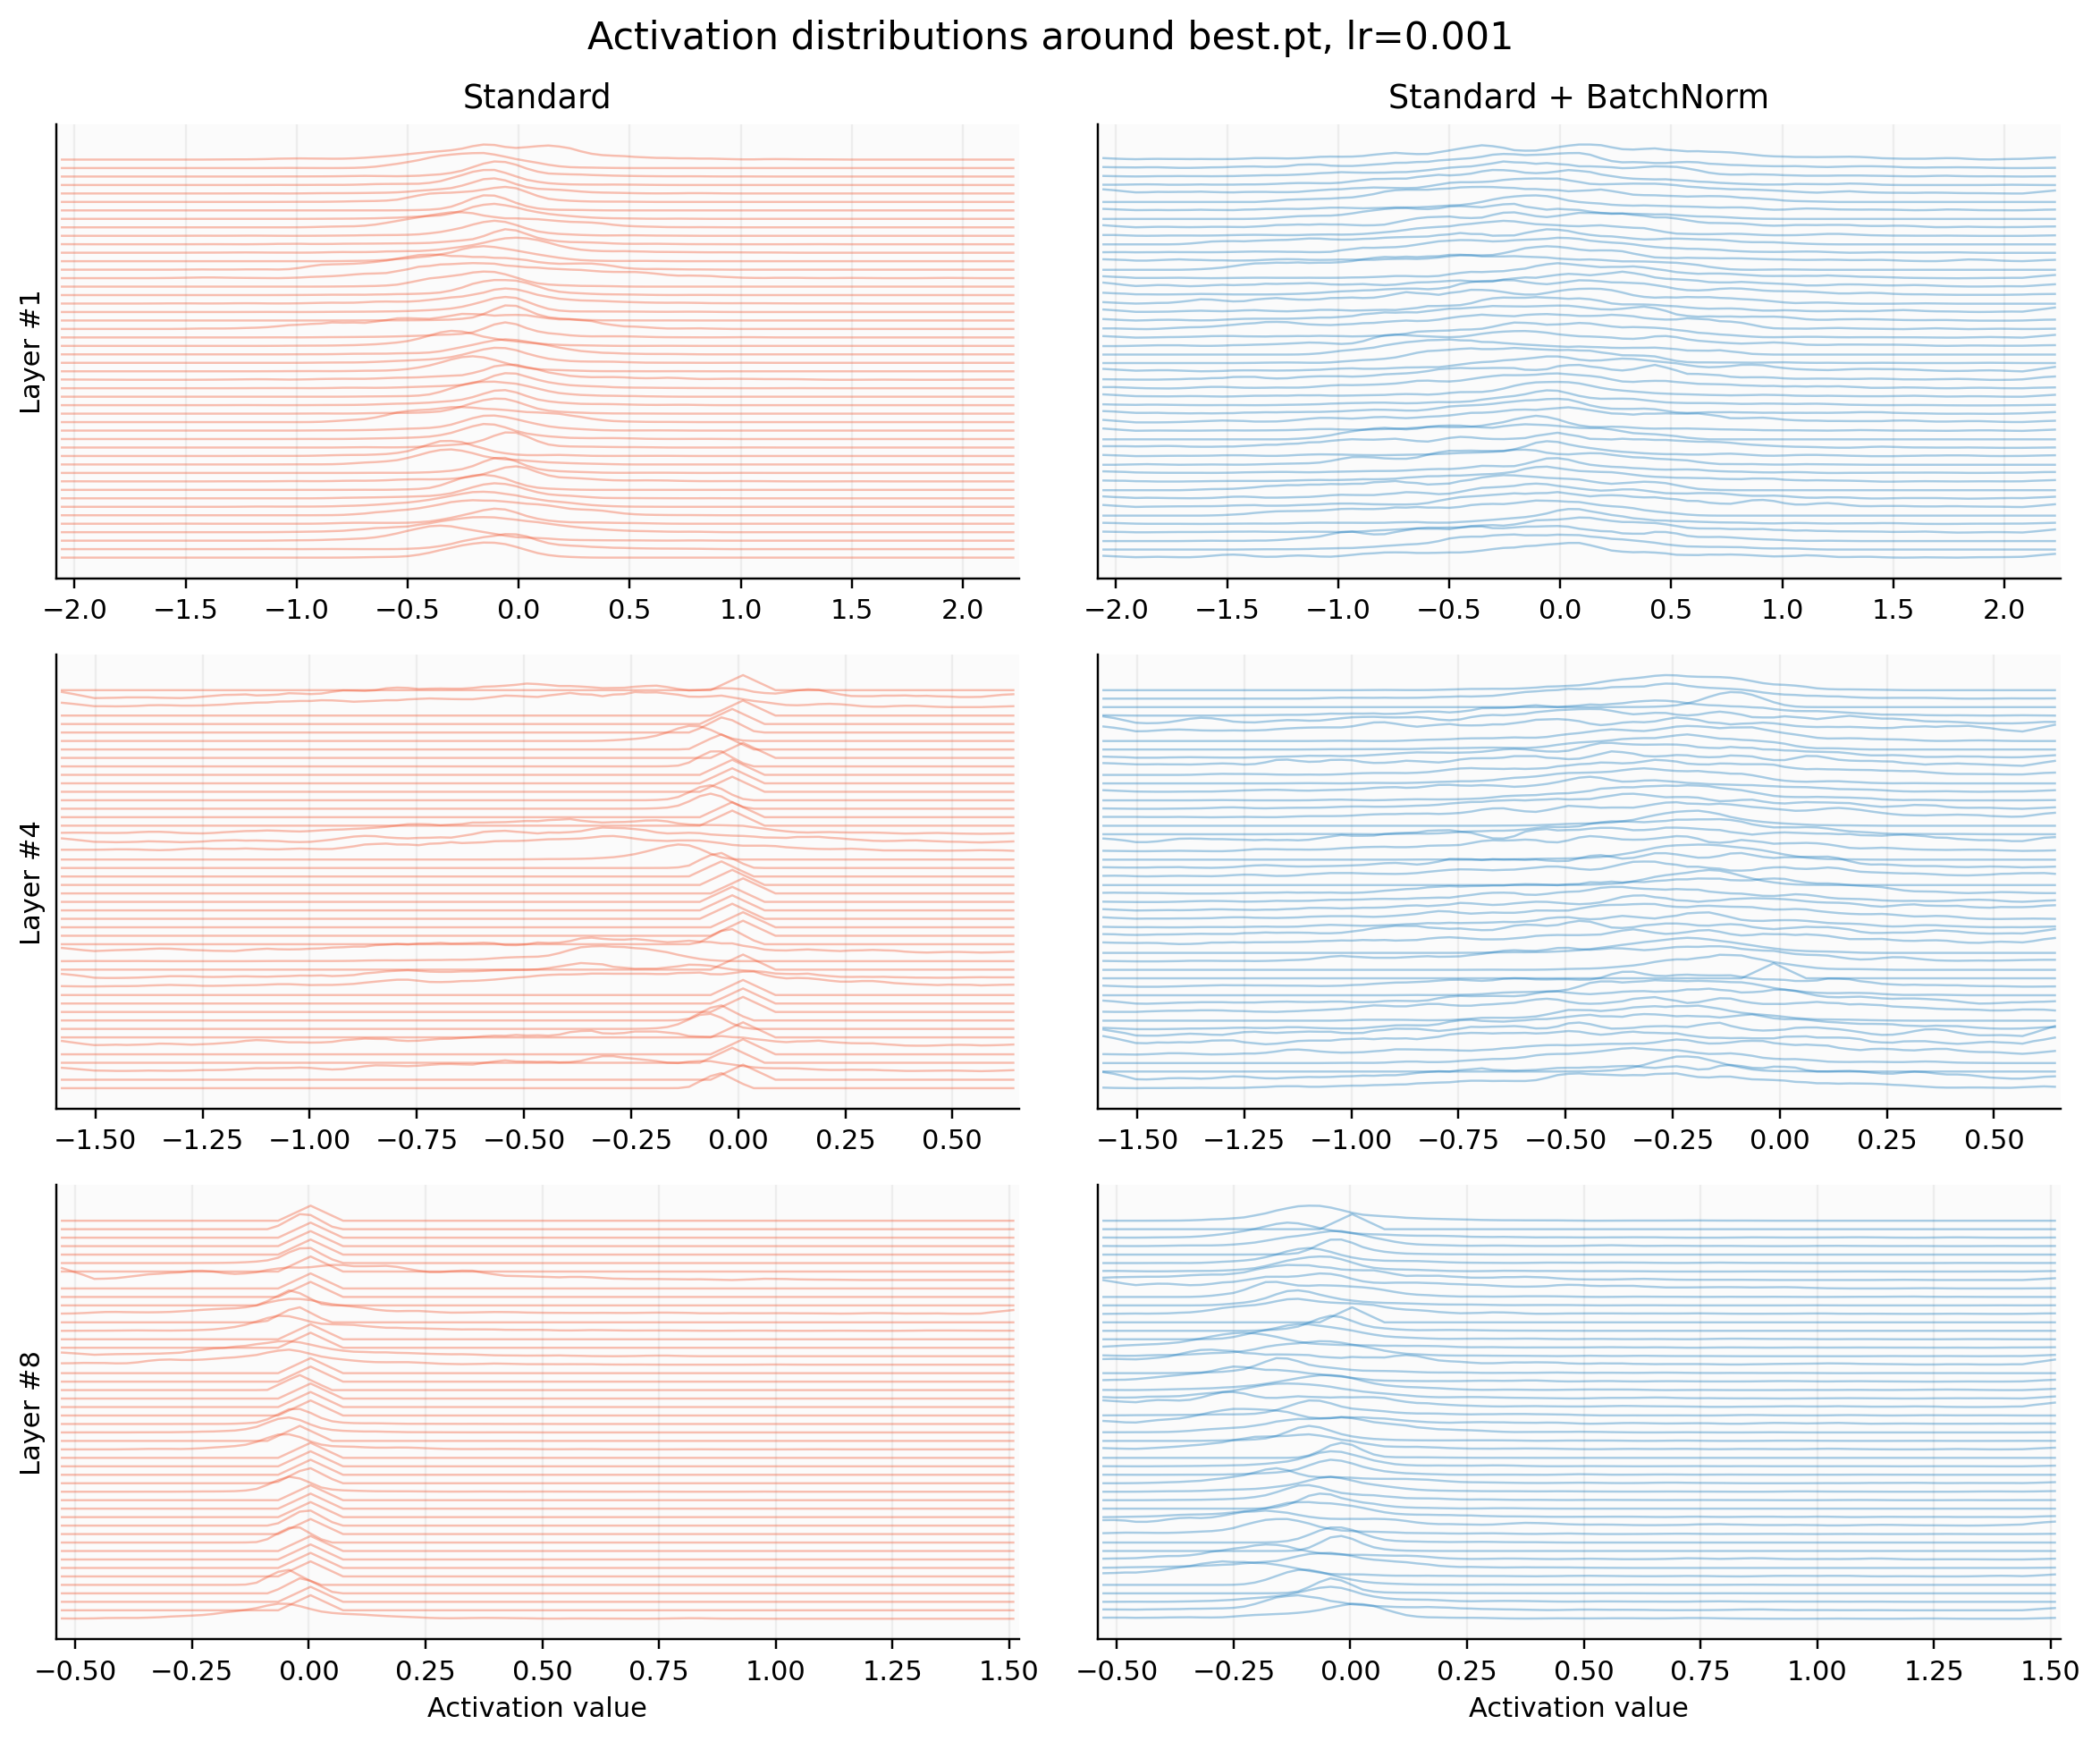
\includegraphics[width=0.95\linewidth]{activation_distribution_ridgeline.png}
  \caption{不同层的激活分布 ridgeline 图。左列为标准 VGG-A，右列为 VGG-A-BN。BN 后激活在多个层上呈现更宽且更连续的通道分布形态。}
  \label{fig:activation_distribution}
\end{figure}

表~\ref{tab:activation_stats} 给出了对应的激活统计。BN 后激活的标准差在第 1、4、8 层分别为 $0.750$、$0.387$、$0.326$，大于 no-BN 的 $0.268$、$0.275$、$0.146$。这并不矛盾，因为图中采集的是训练完成后的 BN 输出，而不是训练过程中每个 batch 的 pre-BN 到 post-BN 归一化瞬间；BN 的可学习 $\gamma,\beta$ 会重新缩放和平移激活。更重要的是，BN 提供了受控的通道级重参数化，使网络可以在训练中学习合适尺度，而不是让每层输入分布完全由前面层的权重漂移决定。

\begin{table}[H]
  \centering
  \caption{激活分布统计}
  \label{tab:activation_stats}
  \begin{tabular}{cccccc}
    \toprule
    模型 & 层 & 均值 & 标准差 & 1\% 分位 & 99\% 分位 \\
    \midrule
    VGG-A & 1 & $-0.125$ & $0.268$ & $-0.846$ & $0.653$ \\
    VGG-A & 4 & $-0.117$ & $0.275$ & $-1.273$ & $0.227$ \\
    VGG-A & 8 & $-0.004$ & $0.146$ & $-0.318$ & $0.443$ \\
    VGG-A-BN & 1 & $-0.095$ & $0.750$ & $-2.059$ & $2.239$ \\
    VGG-A-BN & 4 & $-0.303$ & $0.387$ & $-1.440$ & $0.627$ \\
    VGG-A-BN & 8 & $-0.015$ & $0.326$ & $-0.504$ & $1.452$ \\
    \bottomrule
  \end{tabular}
\end{table}

\section{综合分析}

\subsection{BN 对性能的影响}

在本实验中，BN 对最终性能的提升主要体现在中等和偏大学习率下。学习率 $10^{-3}$ 时，BN 的最佳验证准确率比 no-BN 高 $4.21$ 个百分点；学习率 $2\times10^{-3}$ 时，差距扩大到 $71.36$ 个百分点。这说明 BN 并不是简单地在所有超参数下稳定提升，而是显著改变了模型对学习率的容忍范围。

小学习率下 BN 并不一定更优。例如 $10^{-4}$ 和 $5\times10^{-5}$ 时，no-BN 的最佳验证准确率分别高于 BN $2.13$ 和 $4.51$ 个百分点。原因可能是小学习率训练本身已经稳定，BN 带来的重参数化优势没有充分体现；同时 BN 引入的 batch 统计噪声、running statistics 误差以及额外仿射参数也可能影响最终泛化。

\subsection{BN 对优化稳定性的影响}

多个证据共同支持 BN 改善优化稳定性：
\begin{enumerate}
  \item Loss 包络显著变窄。BN 的平均包络宽度仅为 $0.375$，无 BN 为 $1.900$。
  \item 学习率 sweep 中，BN 在 $5\times10^{-4}$ 到 $5\times10^{-3}$ 区间均保持 $75\%$ 以上最佳验证准确率，而 no-BN 在 $2\times10^{-3}$ 和 $3\times10^{-3}$ 下失败。
  \item 训练曲线显示 BN 在早期 epoch 更快达到较高验证准确率，说明它改善了优化路径，而不只是后期精调。
  \item 梯度预测性实验显示，在较大学习率下 no-BN 的梯度方向连续性几乎丧失且训练失败，而 BN 仍保持有效学习。
\end{enumerate}

这些结果与 Santurkar 等人在 ``How Does Batch Normalization Help Optimization?'' 中提出的观点一致：BN 的重要作用不是简单减少 internal covariate shift，而是通过重参数化使优化问题更加平滑，从而提高梯度下降类方法的稳定性。

\subsection{局限性}

本实验仍有若干局限。首先，基础训练未使用数据增强，因此最终准确率不能代表 VGG-A 在 CIFAR-10 上的最佳可达性能。其次，loss 包络方法是作业建议的简化度量，它通过不同学习率下训练曲线的范围反映稳定性，并不是严格意义上的全局 Lipschitz 常数估计。第三，三维 loss surface 只是高维参数空间的二维随机切片，不同随机方向可能得到不同视觉形态。最后，梯度预测性指标受训练是否失败影响较大，必须结合准确率、loss 和梯度范数共同解释。

\section{结论}

本部分完成了 VGG-A 与 VGG-A-BatchNorm 在 CIFAR-10 上的系统对比，并从分类性能、训练曲线、loss landscape、学习率敏感性、梯度变化和激活分布等角度分析 BN 的作用。实验结论如下：

\begin{enumerate}
  \item BN 在中等和较大学习率下显著提升 VGG-A 的训练稳定性和验证准确率。最佳结果为 $82.18\%$，高于无 BN 模型的 $79.25\%$ 最高结果。
  \item BN 显著扩大可用学习率范围。无 BN 在 $2\times10^{-3}$ 和 $3\times10^{-3}$ 下退化到 $10\%$，而 BN 分别达到 $81.36\%$ 和 $79.46\%$。
  \item BN 缩小跨学习率 loss 包络，平均包络宽度从 $1.900$ 降至 $0.375$，说明训练 loss 对学习率变化更不敏感。
  \item 梯度预测性与可视化实验进一步表明，BN 改善的是训练过程中的优化动态，而不仅仅是最终分类器的表达能力。
\end{enumerate}

因此，在本实验设置下，Batch Normalization 的核心价值可以概括为：通过通道级归一化和可学习重参数化，稳定深层网络的训练过程，使优化景观在实际训练路径上更加平滑，并显著提高模型对学习率选择的鲁棒性。

\begin{thebibliography}{9}
\bibitem{ioffe2015batch}
Sergey Ioffe and Christian Szegedy.
\newblock Batch Normalization: Accelerating Deep Network Training by Reducing Internal Covariate Shift.
\newblock ICML, 2015.

\bibitem{santurkar2018how}
Shibani Santurkar, Dimitris Tsipras, Andrew Ilyas, and Aleksander Madry.
\newblock How Does Batch Normalization Help Optimization?
\newblock NeurIPS, 2018.

\bibitem{cifar10}
Alex Krizhevsky.
\newblock Learning Multiple Layers of Features from Tiny Images.
\newblock Technical report, 2009.
\end{thebibliography}

\end{document}
